%
\section{PDDL}
\label{sect:PDDL}
The objective behind domain independent planning is to formulate a
planner that is able to construct plans across a wide variety of planning domains with 
no change to the planning algorithms. The typical problem presented to such a planner
consists of:
%
\begin{itemize}
\item A set of objects,
\item A set of predicate expressions that define properties of
objects and relations between objects,
\item A set of actions that are able to manipulate the predicate
expressions,
\item A set of predicate expressions that constitute a partial
world state and make up the initial conditions,
\item A set of problem goals, which are predicate expressions that are required to be 
true at the end of a plan.
\end{itemize}
%
If an {\it action} is defined as a fully-instantiated operator, then the job of the planner is to formulate a sequential list of valid actions, referred to as a {\it valid plan}, which will bring the system from the state represented by the initial conditions to a state that satisfies the problem goals (all of the problem goals are simultaneously true).
%
\begin{figure}[htb!]
\begin{center}
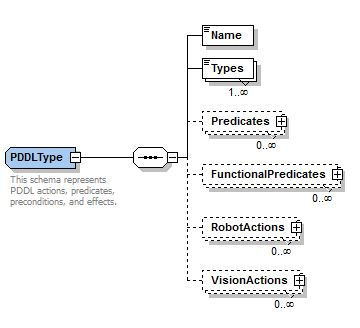
\includegraphics[width=8.5cm]{images/PDDLType.jpg}
\caption{Description of the PDDLType class that is designed as
an augmented PDDL description language. It contains all of the
information necessary for interacting with the robot cell's
robot controller and vision system.}
\label{fig:pddlType}
\end{center}
\end{figure}
%

PDDL is designed as a standard language and structure for 
representing a valid plan along with all of the elements of
domain independent planning systems. Figure \ref{fig:pddlType}
depicts a schema view of our augmented PDDL representation.
As in a standard PDDL representation, a set of object {\it types} 
is represented along with \textit{predicate} expressions and 
{\it actions}. The schema has been augmented with the
representation of \textit{functionalPredicates} and
the distinction between \textit{RobotActions} and
\textit{VisionActions}.

In PDDL, {\it types} must be declared before their use as
parameters to predicate expressions. For our PDDL extension,
the additional requirement has been added that all types must
be defined in the system's ontology and must be derived from the base
\textit{SolidObject} or \textit{SystemConstant}
classes. This assures that basic properties of
objects being used as parameters are known to the system.
The \textit{SolidObject} provides the basis for all physical
objects in the world while the \textit{SystemConstant}
represents a named system memory location that may be used as intermediate 
storage of values between commands. It is often used by \textit{VisionActions}
to store values required by a future \textit{RobotAction}.

\textit{Predicates} are binary expressions that contain one or 
two objects
of defined \textit{types} as arguments and provide a partial 
definition of the world's state. Predicates may be used for 
\textit{preconditions} (predicates that must be true for an
action to be executed) as well as \textit{effects} (predicates
that are expected to become true as the result of an action).
An additional class of predicates known as \textit{FunctionalPredicates}
has been added to this representation. These predicates allow for
mathematical operations to be performed between parameters. For example,
the predicate \textit{equalTo(obj1, value)} will evaluate the
equivalence between \textit{obj1} and \textit{value} while the predicate
\textit{set-value(systemVariable, setValue, valueType)} will set the value of the variable 
\textit{systemVariable} to \textit{setValue}. The \textit{set-value} predicate
will evaluate to \textit{true} if the memory location to be set exists and the value
to be set is of the correct type for that memory location.

\textit{Actions} represent compound tasks that the robot cell must accomplish.
Our robot cell consists of a robotic arm and a vision system. Therefore, our
actions have been segregated into \textit{RobotActions} that pertain to the robot system
and \textit{VisionActions} that pertain to the vision system.
More information on the implementation of these types in the ontology may be found in Section \ref{sect:knowledge}. 
